\subsubsection{Visitor}
\label{ssub:visitor}

Rappresenta un'operazione da svolgersi sugli elementi di una struttura di
oggetti. Il pattern Visitor permette di definire una nuova operazione senza
cambiare la classe degli elementi su cui opera.

Con il pattern Visitor si hanno due gerarchie separate: una per gli elementi su
cui si va a operare e una per i visitor, che definiscono le operazioni su tali
elementi. Per aggiungere una nuova operazione si aggiunge una classe alla
gerarchia di visitor.

\paragraph{Applicabilità}
\label{par:applicabilit_}

Si può applicare il Visitor quando:

\begin{itemize}
  \item una struttura di oggetti contiene classi di oggetti con interfacce
  differenti, e si vogliono eseguire delle operazioni su tali oggetti che
  dipendono dalle loro classi concrete;
  \item è necessario eseguire diverse operazioni non correlate tra loro su
  alcuni oggetti di una struttura, e si vuole evitare di ``sporcare'' tali
  classi con queste operazioni;
  \item le classi che definiscono la struttura cambiano raramente, ma interessa
  cambiare le operazioni su di esse.
\end{itemize}

\begin{figure}[h!]
  \centering
  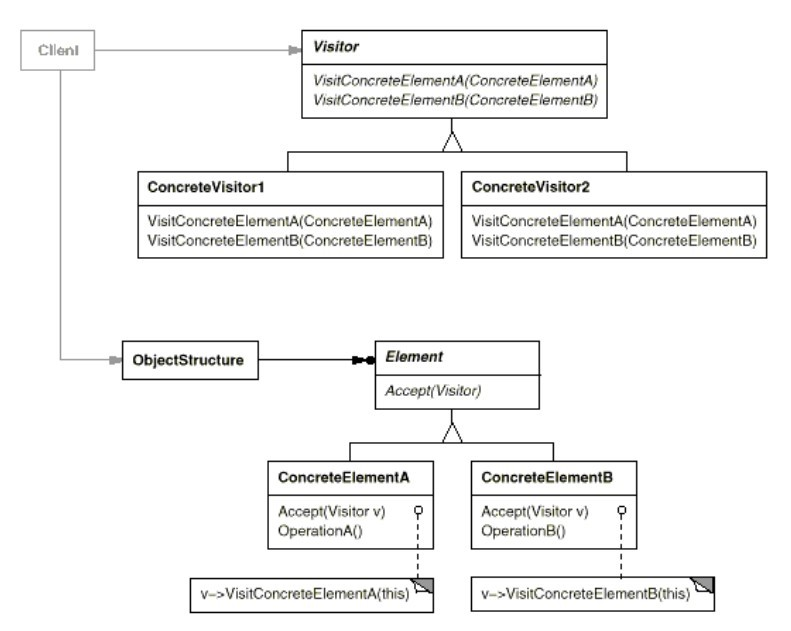
\includegraphics[scale=0.5]{imgs/visitor}
  \caption{Diagramma delle classi del pattern Visitor}
\end{figure}

\paragraph{Partecipanti}
\label{par:partecipanti}

\begin{description}
  \item[Visitor] Dichiara un metodo `visit' per ogni classe concreta della
  struttura. Il nome del metodo e la sua firma identificano la classe
  dell'oggetto che invia la richiesta di visita al Visitor;
  \item[ConcreteVisitor] Ogni visitor concreto implementa i metodi definiti
  dalla classe astratta relativa ad ogni classe della struttura, e rappresenta
  una particolare operazione sugli oggetti della struttura;
  \item[Element] Definisce un metodo accept() che prende un visitor per
  argomento;
  \item[ConcreteElement]
  \item[ObsectStructure] \`E in grado di enumerare sugli elementi.
\end{description}

Un client che utilizza il pattern Visitor deve creare un oggetto Visitor
concreto e traversare gli oggetti della struttura, passando il visitor ad ognuno
di essi.

\paragraph{Conseguenze}
\label{par:conseguenze}

\begin{itemize}
  \item Il pattern facilita l'aggiunta di nuove operazioni: per definire una
  nuova operazione è sufficiente definire una nuova classe visitor concreta;
  \item Il pattern Visitor raggruppa operazioni correlate e separa quelle non
  correlate. Questo semplifica sia le classi degli elementi sia quelle degli
  algoritmi, e permette di nascondere ogni dato specifico di un algoritmo nella
  relativa classe;
  \item Aggiungere nuove classi alla gerarchia di elementi è difficile, e
  richiede la modifica dell'intera gerarchia di Visitor. Per questo, è
  consigliabile utilizzare il pattern solamente quando le operazioni sugli
  elementi possono variare, ma non gli elementi stessi;
  \item Il Visitor può traversare strutture di oggetti indipendentemente dalla
  loro gerarchia. Mentre un Iterator può attraversare solamente oggetti con una
  classe base comune, il Visitor non soffre di questo vincolo;
  \item Il Visitor è in grado di accumulare stato man mano che traversa la
  struttura di oggetti;
  \item Il pattern Visitor è in realtà un anti-pattern in quanto incentiva la
  \strong{rottura dell'incapsulazione}, uno dei principi fondamentali del
  paradigma ad
  oggetti.
\end{itemize}

% paragraph conseguenze (end)
